\documentclass{article}
\usepackage[T1]{fontenc}
\usepackage{lmodern}
\usepackage{graphicx}
\usepackage{amsmath,amssymb}
\usepackage[a4paper,margin=2cm]{geometry}
\usepackage[absolute,overlay]{textpos}
\setlength{\TPHorizModule}{1mm}
\setlength{\TPVertModule}{1mm}
\usepackage[indonesian]{babel}
\usepackage{hyperref}
\setlength{\emergencystretch}{2em}
% unit: Halaman 11

\begin{document}

% === Halaman 11 (llm) ===

\vspace{10mm}

Gambar 3. Pembangkitan kunci internal

% deskripsi: Diagram alir proses pembangkitan kunci internal DES yang menunjukkan langkah-langkah dari Kunci eksternal 64 bit, melalui Permutasi PC-1, pembagian menjadi C dan D (masing-masing 28 bit), proses Left Shift berulang, hingga Permutasi PC-2 untuk menghasilkan kunci internal K1 sampai K16 dengan panjang 48 bit.
% bbox normalisasi: [0.0500, 0.1000, 0.6800, 0.9600]
\begin{textblock*}{132.30mm}(10.50mm,29.70mm)
\noindent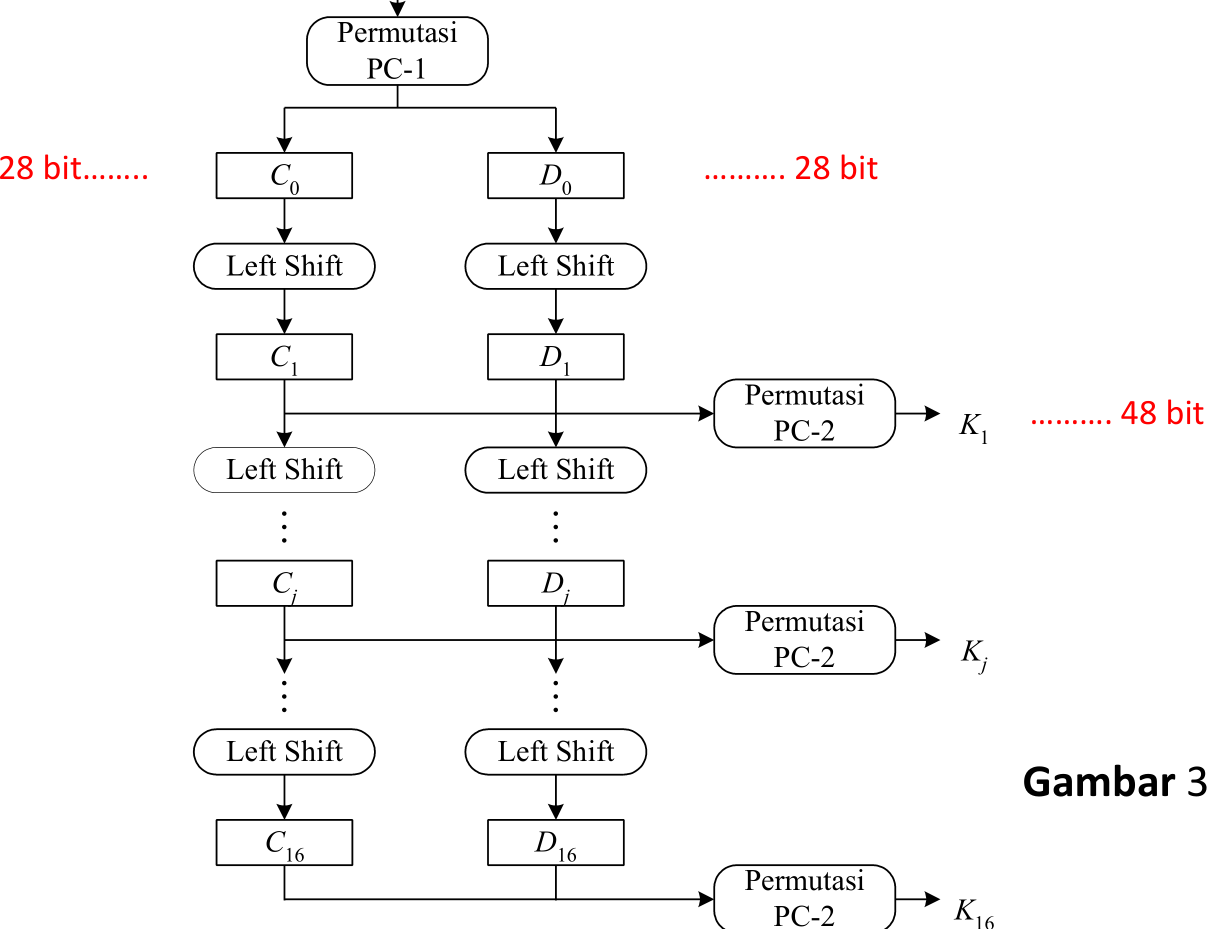
\includegraphics[width=132.30mm,height=255.42mm]{../../images/llm/page_011_img_01.png}%
\end{textblock*}

\end{document}
